\NeedsTeXFormat{LaTeX2e}

\documentclass{cje_appendix} % for use when submitting final paper for publication
  \usepackage{cjenatbib}
  \usepackage{url}
   
%  \ifx\pdftexversion\undefined
%    \usepackage[dvips]{graphicx}
%  \else
%    \usepackage[pdftex]{graphicx}
%    \usepackage{epstopdf}
%    \epstopdfsetup{suffix=}
%  \fi

  \usepackage{tabularx}
  \usepackage[figuresright]{rotating}
  \usepackage{floatpag}
  \rotfloatpagestyle{empty}
  \usepackage{amsmath}
  \usepackage{amsthm}
  \usepackage{amssymb}
\usepackage{amsfonts}
  \theoremstyle{plain}% default
    \newtheorem{theorem}{Theorem}
    \newtheorem{lemma}{Lemma}
    \newtheorem{proposition}{Proposition}
    \newtheorem*{corollary}{Corollary}
  \theoremstyle{definition}
    \newtheorem{definition}{Definition}
    \newtheorem{example}{Example}
  \theoremstyle{remark}
    \newtheorem*{remark}{Remark}
    \newtheorem*{case}{Case}
  \usepackage{lmodern}
  \usepackage{upquote}
\usepackage[printonlyused]{acronym}
 \usepackage{makecell}
 \usepackage[figuresright]{rotating}

\usepackage{longtable}
\usepackage{array}
\usepackage{lscape}
\usepackage{dcolumn}
\usepackage{float}
\usepackage{pdfpages}
\usepackage{rotating}
\usepackage{lscape}
\usepackage{dcolumn}
%\usepackage{csquotes}
\usepackage{etoolbox}
\usepackage{placeins}
\usepackage{csvsimple}
\usepackage{xspace}
\usepackage{tabularx,booktabs}
\usepackage{siunitx} % for 's' column type
\usepackage{comment}
\usepackage{tikz}
\usepackage{xr-hyper}
 \usepackage{hyperref}
\IfFileExists{upquote.sty}{\usepackage{upquote}}{}
\usepackage{graphicx}
\usepackage{flafter}
\usepackage{filecontents}
\usepackage{multibib}
\newcites{supp}{Supplementary References}

 % setting article items used multiple times
\newcommand{\mytitle}{Reproduce to Validate: a Comprehensive Study on the Reproducibility of Economics Research \\  Online Appendix}

\newcommand{\myauthorA}{Hautahi Kingi}
\newcommand{\myauthorB}{Flavio Stanchi}
\newcommand{\myauthorC}{Lars Vilhuber*}
\newcommand{\myauthorD}{Sylv\'erie Herbert}
\authorone{\myauthorD}{Banque de France} %{Full name of author one}{Name of department and organization or institution; separate multiple affiliations with semi-colon}
\authortwo{\myauthorA}{Google} %{Full name of author two}{Name of department and organization or institution; separate multiple affiliations with semi-colon}
\authorthree{\myauthorB}{Airbnb} %{Full name of author three}{Name of department and organization or institution; separate multiple affiliations with semi-colon} 
\authorfour{\myauthorC}{Labor Dynamics Institute, Cornell University}%{Full name of author four}{Name of department and organization or institution; separate multiple affiliations with semi-colon}


\renewcommand\theadalign{bl}

   %To enable possessive citations (using \citeapos)
\def\citeapos#1{\citeauthor{#1}'s (\citeyear{#1})}
 
 %If you have landscape tables or figures
\usepackage[figuresright]{rotating}
\usepackage{floatpag}
  \rotfloatpagestyle{empty}

  \hypersetup{%
    pdftitle = {\mytitle},
pdfauthor={\myauthorD, \myauthorA, \myauthorB, \myauthorC},%
    citecolor=blue,            
    urlcolor=blue,
    colorlinks = true,
  }  	  

  \bibpunct{(}{)}{,}{a}{}{;}
  
\externaldocument[]{cjetemplate}


\begin{document}
\title[]{Reproduce to Validate: a Comprehensive Study on the Reproducibility of Economics Research \\  Online Appendix} %For running heads. [short running title (max. 40 characters if possible)]{full title}
\authors{} %Summary of authors for running heads. {Author initials and family names separated by commas except before ``and''}
\acknowledgements{Corresponding author: lars.vilhuber@cornell.edu.}

\maketitle
\clearpage
\appendix

\section{Appendix}\label{sec:app}
\subsection{Appendix Tables}\label{sec:app:tables}
\begin{table}
\centering
\caption{Assignments by publication year} 
\label{tab:assignments}
\begin{tabular}{rrrrrr}
  &\multicolumn{5}{c}{Assignment Years}\\ & 2015 & 2016 & 2017 & 2018 & 2019 \\ 
  \hline
2009 &   0 &  23 &   3 &   1 &   0 \\ 
  2010 &  32 &   6 &   1 &   0 &   0 \\ 
  2011 &  36 &   9 &   1 &   0 &   0 \\ 
  2012 &   0 &  41 &   1 &   5 &   0 \\ 
  2013 &   0 &  12 &   1 &   0 &   0 \\ 
  2014 &   0 &   0 &  41 &   5 &   0 \\ 
  2015 &   0 &   0 &   0 &  24 &   0 \\ 
  2016 &   0 &   0 &   0 &  36 &   0 \\ 
  2017 &   0 &   0 &   0 &  43 &   0 \\ 
  2018 &   0 &   0 &   0 &  20 &   1 \\ 
   \hline
\end{tabular}
\end{table}


 \begin{sidewaystable} \centering 
\scriptsize
  \caption{Assessment of Data Availability, By Year} 
  \label{tab:absence} 
\begin{tabular}{@{\extracolsep{0.4pt}} ccccccccccccc} 
\\[-1.8ex]\hline 
\hline \\[-1.8ex] 
Reason & 2009 & 2010 & 2011 & 2012 & 2013 & 2014 & 2015 & 2016 & 2017 & 2018 & Total & Percent \\ 
\hline \\[-1.8ex] 
Confidential Data & 5 & 10 & 8 & 11 & 1 & 17 & 2 & 12 & 12 & 8 & 86 & 31.39 \\ 
Data was Provided & 14 & 13 & 24 & 26 & 7 & 23 & 18 & 20 & 26 & 9 & 180 & 65.69 \\ 
No Data or Reason & 2 & 0 & 0 & 2 & 0 & 0 & 1 & 1 & 1 & 1 & 8 & 2.92 \\ 
Total & 21 & 23 & 32 & 39 & 8 & 40 & 21 & 33 & 39 & 18 & 274 & 100 \\ 
\hline \\[-1.8ex] 
\multicolumn{13}{l}{\footnotesize Notes: Assessments made  by replicators using the entry questionnaire, prior to attempting reproduction.} \\ 
\end{tabular} 
 \end{sidewaystable}



\FloatBarrier
\begin{table} \centering 
  \caption{Reproduction Results} 
  \label{tab:results:year} 
\begin{tabular}{@{\extracolsep{0.4pt}} cccccc} 
\\[-1.8ex]\hline 
\hline \\[-1.8ex] 
Year & Successful & Partial & Confidential Data & Other failure & Total \\ 
\hline \\[-1.8ex] 
2009 & 4 & 4 & 5 & 1 & 14 \\ 
2010 & 7 & 3 & 2 & 1 & 13 \\ 
2011 & 10 & 2 & 5 & 7 & 24 \\ 
2012 & 8 & 13 & 2 & 3 & 26 \\ 
2013 & 4 & 3 &  &  & 7 \\ 
2014 & 7 & 11 & 3 & 2 & 23 \\ 
2015 & 4 & 12 & 2 &  & 18 \\ 
2016 & 8 & 7 & 4 & 1 & 20 \\ 
2017 & 13 & 8 & 3 & 2 & 26 \\ 
2018 & 3 & 3 & 2 & 1 & 9 \\ 
Total & 68 & 66 & 28 & 18 & 180 \\ 
Percent & 37.8\% & 36.7\% & 15.6\% & 10\% & 100\% \\ 
\hline \\[-1.8ex] 
\end{tabular} 
\end{table} 
\FloatBarrier
%
\begin{table} \centering 
  \caption{Probit: Determinants of Reproducibility, Year 0} 
  \label{reg:probit:reproducibility:fullpartial:0} 
\begin{tabular}{@{\extracolsep{-15pt}}lD{.}{.}{-3} D{.}{.}{-3} D{.}{.}{-3} } 
\\[-1.8ex]\hline 
\hline \\[-1.8ex] 
\\[-1.8ex] & \multicolumn{3}{c}{Outcome: Full or Partial Reproduction} \\ 
\\[-1.8ex] & \multicolumn{1}{c}{(1)} & \multicolumn{1}{c}{(2)} & \multicolumn{1}{c}{(3)}\\ 
\hline \\[-1.8ex] 
 `Avg. H-index` & 0.0004 &  & 0.081 \\ 
  & (0.021) &  & (0.099) \\ 
  `Max H-index` &  & -0.002 & -0.032 \\ 
  &  & (0.011) & (0.039) \\ 
  `Highest Institution Publications` & -0.011 & -0.012 &  \\ 
  & (0.009) & (0.009) &  \\ 
  `Min H-index` &  &  & -0.021 \\ 
  &  &  & (0.067) \\ 
  `Institution Publications (top)` &  &  & -0.382 \\ 
  &  &  & (0.596) \\ 
  `Institution Publications (bottom)` &  &  & 4.240 \\ 
  &  &  & (349.000) \\ 
  `Highest Co-author Experience` & -0.024 & -0.023 & -0.026 \\ 
  & (0.019) & (0.018) & (0.023) \\ 
  `Number of authors` & 0.136 & 0.147 & 0.395 \\ 
  & (0.177) & (0.188) & (0.279) \\ 
  `Author at US university` & 0.273 & 0.278 & 0.057 \\ 
  & (0.476) & (0.477) & (0.479) \\ 
  `Solo-authored` &  &  & 0.856 \\ 
  &  &  & (0.715) \\ 
  Constant & 1.680^{***} & 1.670^{***} & 0.823 \\ 
  & (0.529) & (0.535) & (0.946) \\ 
 \textit{N} & \multicolumn{1}{c}{113} & \multicolumn{1}{c}{113} & \multicolumn{1}{c}{113} \\ 
\hline 
\hline \\[-1.8ex] 
\multicolumn{4}{l}{$^{***} p< 0.01$, $^{**} p< 0.05$, $^{*} p < 0.1$} \\ 
\multicolumn{4}{l}{Sample restricted to articles published in 2012 and later, with attempted reproduction.} \\ 
\end{tabular} 
\end{table} 
%
\begin{table} \centering 
  \caption{Publication and Author Metrics (2012+)} 
  \label{tab:metrics:OA:zero} 
\begin{tabular}{@{\extracolsep{0.4pt}} ccccc} 
\\[-1.8ex]\hline 
\hline \\[-1.8ex] 
  & Confidential data & Unsuccessful & Partial & Successful \\ 
\hline \\[-1.8ex] 
Avg h-index & 12.06 & 14.67 & 11.68 & 14.04 \\ 
Lowest h-index & 6.21 & 7.33 & 6.14 & 7.4 \\ 
Number of Authors & 2.27 & 2.44 & 2.32 & 2.6 \\ 
Citations & 2.87 & 2.11 & 3.58 & 5.47 \\ 
Highest experience & 20.57 & 24.89 & 19.28 & 21.53 \\ 
Institutional productivity & 19.63 & 27.85 & 18.48 & 21.47 \\ 
Percent of authors in US & 82.14 & 77.78 & 71.93 & 82.98 \\ 
N & 84 & 9 & 57 & 47 \\ 
\hline \\[-1.8ex] 
\multicolumn{5}{l}{Notes: All assessed articles published after 2011, except for 1 author dropped } \\ 
\multicolumn{5}{l}{for inconsistent OA data.with . Author and institutional characteristics are measured } \\ 
\multicolumn{5}{l}{in the year of publication. } \\ 
\multicolumn{5}{l}{Institutional (cumulative) productivity measured in 10,000 publications.} \\ 
\end{tabular} 
\end{table} 
%
\FloatBarrier

\clearpage
%===================== Supporting lists ======================

\FloatBarrier
\section{Sample directory change}
\label{app:directorychg}

\begin{figure}
\caption{Example of change to author-provided file\label{fig:svndiff}}
\begin{verbatim}
> svn diff -r961:HEAD $SVNURL/10.1257/app.5.4.92/replication-xxx/Data/
 do_files/main_analysis.do
Index: main_analysis.do
===================================================================
--- main_analysis.do	(revision 961)
+++ main_analysis.do	(revision 3425)
@@ -6,7 +6,7 @@
     version 11.2

 *place path here:
-global path "C:\"
+global path "\\rschfs1x\usercl\spring\xxx\Data"
 cd            "$path\output"
 use "$path\data\thefts_sales.dta",clear
 cap log close

\end{verbatim}
\end{figure}


\FloatBarrier

%=============================================================
%               Comparison WoS - OpenAlex

\section{Comparison of bibliometric sources}
\label{app:wos-openalex}


\subsection{Web of Science}

In an earlier version of this paper, we had used data from Web of Science \citep[WoS]{WebofScience}.
We manually queried the WoS  database citations for each article by entering the partial DOI of articles in an issue of AEJ:AE. For later issues, the DOI structure changed, and alternate search criteria were used. For each search results, WoS provided year-by-year citations, as well as total and average citations. We did this in 2015, 2017, and after the conclusion of the exercise, in 2019.

For each of up to five authors per article, we also (contemporaneously) queried WoS, searching for that author, and recording their h-index \citep{Hirsch2005} and the underlying number of citations for each author by year, as well as the search criteria used to find the author. In some cases, a simple search by author name does not yield a unique person (e.g.,  ``Smith, Adam''), and sometimes, the metadata in Web of Science contained errors.
%\footnote{For example, we only found one article for ``Lawrence E. Katz'' in Web of Science as of January 2016, namely the article in \ac{AEJ:AE} \citep{10.1257/app.2.3.228}, but did find quite a few more for ``Lawrence F. Katz.'' While we initially thought this to be the result of some inside joke for senior economists, even the \ac{AEJ:AE} website displays the author of the article (correctly) as ``Lawrence F. Katz,'' and we have no explanation for how this error could persist in the Web of Science database (the error is still present in 2023). Our search criteria adjusted for this error.} 

We adjusted total citations as reported for years since publication (which differed for each issue), and used that adjusted number in our analysis. Results in \cite{kingi2018,herbert2021} relied on these numbers. By design, we excluded several years worth of articles from these analyses, since not enough time had elapsed since the article had been published.

\subsection{OpenAlex}

In response to a referee, we investigated expanding the measurement again, for a larger set of articles over a larger expanse of time. The very manual process combined with an absence of research participants and authors working on this project suggested an alternative approach, which had become feasible in the interim, thanks to the efforts of \cite{openalex2022}. We therefore queried the OpenAlex (OA) corpus \citep{ourresearch2023} via the openly accessible \ac{API}. Code to do so is included in the replication package. 

Generically, OA has more works than WoS. To facilitate the comparison, when computing as-of-year h-index, we remove a few types of works that are not usually encountered on WoS or for that matter on Google Scholar (GS): "\texttt{other}", "\texttt{paratext}", "\texttt{peer-review}", "\texttt{reference-entry}". 

For the 1114 authors in our sample, we identified 506. The median institution is recorded as having published 17614 as of 2023. Cornell University, an R1 research university, is recorded as having published 334943, whereas Wellesley College, a liberal arts college focused on teaching undergraduates, is listed with 9023 works. 

\subsection{Comparison}

No two bibliometric data sources are identical, and we observe certain differences in these two databases as well. This is also true of different snapshots of the same database over time, even for data that ostensibly refers to citations occurring several years back. Thus, variability is to be expected. 

In this section, we compare our subsample of the two databases, for the same articles and authors, where possible. Table~\ref{tab:metrics} is for the smaller sample with manually collected WoS data. Table~\ref{tab:metrics:OA:WoS} reproduces Table~\ref{tab:metrics:OA} in the main text, matched to the WoS extract, but collected at a later stage.


\begin{table} \centering 
  \caption{Publication and Author Metrics, WoS} 
  \label{tab:metrics} 
\begin{tabular}{@{\extracolsep{0.4pt}} cccc} 
\\[-1.8ex]\hline 
\hline \\[-1.8ex] 
  & Unsuccessful & Partial & Successful \\ 
\hline \\[-1.8ex] 
Avg h-index & 7.14 & 7.22 & 7.78 \\ 
Lowest h-index & 5.07 & 4.25 & 4.51 \\ 
Number of Authors & 2.14 & 2.4 & 2.58 \\ 
Citations & 4.04 & 3.6 & 5.26 \\ 
N & 14 & 52 & 45 \\ 
\hline \\[-1.8ex] 
\multicolumn{4}{l}{Notes: Articles with attempted reproduction.} \\ 
\multicolumn{4}{l}{Bibliometric data manually queried from WoS.} \\ 
\end{tabular} 
\end{table} 

\begin{table} \centering 
  \caption{Publication and Author Metrics for WoS sample} 
  \label{tab:metrics:OA:WoS} 
\begin{tabular}{@{\extracolsep{0.4pt}} cccc} 
\\[-1.8ex]\hline 
\hline \\[-1.8ex] 
  & Unsuccessful & Partial & Successful \\ 
\hline \\[-1.8ex] 
Avg h-index & 20.76 & 17.84 & 19.65 \\ 
Lowest h-index & 14.57 & 10.38 & 10.73 \\ 
Number of Authors & 2.14 & 2.42 & 2.58 \\ 
Citations & 7.07 & 8.56 & 12.04 \\ 
Highest experience & 25.79 & 23.4 & 25.27 \\ 
Institutional productivity & 26.57 & 18.12 & 23.2 \\ 
Percent of authors in US & 71.43 & 73.08 & 82.22 \\ 
N & 14 & 52 & 45 \\ 
\hline \\[-1.8ex] 
\multicolumn{4}{l}{Notes: Assessed articles matched to Web of Science database extract. Author } \\ 
\multicolumn{4}{l}{and institutional characteristics are measured 4 years after publication.} \\ 
\multicolumn{4}{l}{Institutional (cumulative) productivity measured in 10,000 publications.} \\ 
\end{tabular} 
\end{table} 

In general, the absolute level of citations and derivative h-indexes are much higher in OA. In both databases, however, the approximate relative levels are similar.


\clearpage

\section{Summary statistics}
\label{app:sumstat}
Tables~\ref{tab:statdesc:attemped} and ~\ref{tab:statdesc:assessed} present the summary statistics for the two main samples used in our regressions. The first one concerns assessed articles, based on complete entry questionnaires, and the second are articles for which reproduction was attempted.
\FloatBarrier
\begin{table} \centering 
  \caption{Summary statistics} 
  \label{tab:statdesc:assessed} 
\begin{tabular}{@{\extracolsep{0.4pt}}lD{.}{.}{-3} D{.}{.}{-3} D{.}{.}{-3} D{.}{.}{-3} D{.}{.}{-3} } 
\\[-1.8ex]\hline 
\hline \\[-1.8ex] 
Statistic & \multicolumn{1}{c}{N} & \multicolumn{1}{c}{Mean} & \multicolumn{1}{c}{St. Dev.} & \multicolumn{1}{c}{Min} & \multicolumn{1}{c}{Max} \\ 
\hline \\[-1.8ex] 
Fully reproduced & 180 & 0.378 & 0.486 & 0 & 1 \\ 
Full or Partial & 180 & 0.761 & 0.428 & 0 & 1 \\ 
AsinH(YTD citations) & 273 & 4.040 & 0.886 & 0.000 & 6.540 \\ 
Avg. H-index & 273 & 16.400 & 11.000 & 1.000 & 63.000 \\ 
Max H-index & 273 & 24.800 & 20.400 & 1 & 133 \\ 
Min H-index & 273 & 9.360 & 7.340 & 1 & 52 \\ 
\hline \\[-1.8ex] 
\multicolumn{6}{l}{Notes: } \\ 
\multicolumn{6}{l}{Full or partial reproduction are defined in the text.} \\ 
\multicolumn{6}{l}{Results for all articles with complete assessment.} \\ 
\end{tabular} 
\end{table} 
\FloatBarrier
\begin{table} \centering 
  \caption{Summary statistics} 
  \label{tab:statdesc:attemped} 
\begin{tabular}{@{\extracolsep{0.4pt}}lD{.}{.}{-3} D{.}{.}{-3} D{.}{.}{-3} D{.}{.}{-3} D{.}{.}{-3} } 
\\[-1.8ex]\hline 
\hline \\[-1.8ex] 
Statistic & \multicolumn{1}{c}{N} & \multicolumn{1}{c}{Mean} & \multicolumn{1}{c}{St. Dev.} & \multicolumn{1}{c}{Min} & \multicolumn{1}{c}{Max} \\ 
\hline \\[-1.8ex] 
Fully reproduced & 180 & 0.378 & 0.486 & 0 & 1 \\ 
Full or Partial & 180 & 0.761 & 0.428 & 0 & 1 \\ 
AsinH(YTD citations) & 180 & 4.060 & 0.875 & 0.881 & 6.540 \\ 
Avg. H-index & 180 & 16.800 & 11.100 & 1.000 & 63.000 \\ 
Max H-index & 180 & 25.500 & 20.900 & 1 & 133 \\ 
Min H-index & 180 & 9.710 & 7.630 & 1 & 52 \\ 
\hline \\[-1.8ex] 
\multicolumn{6}{l}{Notes: } \\ 
\multicolumn{6}{l}{Full or partial reproduction are defined in the text.} \\ 
\multicolumn{6}{l}{Results for all articles with attempted reproduction.} \\ 
\end{tabular} 
\end{table} 
\FloatBarrier


\section{Alternative specifications}
\label{app:altspec}
\subsection{Alternative specifications of the link between citation count, reproducibility and hindex}

\subsubsection{Levels, log, and Poisson regressions}
\begin{table} \centering 
  \caption{OLS: YTD Citations on Reproduction Outcomes } 
  \label{reg3:OA} 
\begin{tabular}{@{\extracolsep{-20pt}}lD{.}{.}{-3} D{.}{.}{-3} D{.}{.}{-3} D{.}{.}{-3} } 
\\[-1.8ex]\hline 
\hline \\[-1.8ex] 
\\[-1.8ex] & \multicolumn{1}{c}{(1)} & \multicolumn{1}{c}{(2)} & \multicolumn{1}{c}{(3)} & \multicolumn{1}{c}{(4)}\\ 
\hline \\[-1.8ex] 
 `Avg. H-index` & 0.608 &  &  & 4.500^{***} \\ 
  & (0.373) &  &  & (1.690) \\ 
  `Max H-index` &  & 0.208 &  & -1.870^{**} \\ 
  &  & (0.194) &  & (0.740) \\ 
  `Full or Partial` &  &  &  & -13.800 \\ 
  &  &  &  & (13.700) \\ 
  `Min H-index` &  &  & 0.572 & -1.700 \\ 
  &  &  & (0.533) & (1.340) \\ 
  `Fully reproduced` & -11.500 & -11.200 & 8.230 & 0.477 \\ 
  & (11.600) & (10.400) & (10.400) & (13.000) \\ 
  `Highest Institution Publications` & 0.163 & 0.141 & 0.161 & 0.115 \\ 
  & (0.161) & (0.162) & (0.169) & (0.165) \\ 
  `Highest Co-author Experience` & -0.098 & 0.028 & 0.196 & -0.217 \\ 
  & (0.338) & (0.332) & (0.339) & (0.339) \\ 
  `Number of authors` & 9.400^{**} & 7.640^{**} & 10.400^{***} & 13.100^{***} \\ 
  & (3.630) & (3.710) & (3.850) & (4.110) \\ 
  `Author at US university` & 3.680 & 4.440 & 5.190 & 3.150 \\ 
  & (7.700) & (7.730) & (8.000) & (7.720) \\ 
  `Solo-authored` & 11.500 & 10.900 & 8.600 & 21.000^{*} \\ 
  & (10.100) & (10.100) & (10.500) & (10.800) \\ 
  `Avg. H-index`:`Fully reproduced` & 1.420^{**} &  &  & 0.686 \\ 
  & (0.574) &  &  & (0.671) \\ 
  `Max H-index`:`Fully reproduced` &  & 0.976^{***} &  &  \\ 
  &  & (0.326) &  &  \\ 
  `Min H-index`:`Fully reproduced` &  &  & 0.466 &  \\ 
  &  &  & (0.846) &  \\ 
  `Max H-index`:`Full or Partial` &  &  &  & 0.469 \\ 
  &  &  &  & (0.384) \\ 
  `Full or Partial`:`Min H-index` &  &  &  & -0.452 \\ 
  &  &  &  & (1.070) \\ 
  Constant & -2.850 & 3.060 & -7.530 & -6.180 \\ 
  & (14.200) & (13.900) & (15.000) & (16.600) \\ 
 Observations & \multicolumn{1}{c}{180} & \multicolumn{1}{c}{180} & \multicolumn{1}{c}{180} & \multicolumn{1}{c}{180} \\ 
Adjusted R$^{2}$ & \multicolumn{1}{c}{0.159} & \multicolumn{1}{c}{0.149} & \multicolumn{1}{c}{0.089} & \multicolumn{1}{c}{0.172} \\ 
\hline \\[-1.8ex] 
\multicolumn{5}{l}{$^{***} p< 0.01$, $^{**} p< 0.05$, $^{*} p < 0.1$} \\ 
\multicolumn{5}{l}{Notes: } \\ 
\multicolumn{5}{l}{YTD citations are cumulative citations to the article in Year 4.} \\ 
\multicolumn{5}{l}{H-index measures are computed across all authors of an article, in the previous year.} \\ 
\multicolumn{5}{l}{An author without citations has an h-index of 0. } \\ 
\multicolumn{5}{l}{Full or partial reproduction are defined in the text.} \\ 
\multicolumn{5}{l}{Results for all articles with attempted reproduction.} \\ 
\end{tabular} 
\end{table} 
%\FloatBarrier

\begin{table} \centering 
  \caption{OLS: Log Citations on Reproduction Outcomes } 
  \label{logreg3alt:OA} 
\begin{tabular}{@{\extracolsep{-20pt}}lD{.}{.}{-3} D{.}{.}{-3} D{.}{.}{-3} D{.}{.}{-3} } 
\\[-1.8ex]\hline 
\hline \\[-1.8ex] 
\\[-1.8ex] & \multicolumn{1}{c}{(1)} & \multicolumn{1}{c}{(2)} & \multicolumn{1}{c}{(3)} & \multicolumn{1}{c}{(4)}\\ 
\hline \\[-1.8ex] 
 `Avg. H-index` & 0.023^{***} &  &  & 0.104^{***} \\ 
  & (0.007) &  &  & (0.039) \\ 
  `Max H-index` &  & 0.009^{**} &  & -0.034^{**} \\ 
  &  & (0.004) &  & (0.015) \\ 
  `Min H-index` &  &  & 0.023^{**} & -0.042^{*} \\ 
  &  &  & (0.010) & (0.025) \\ 
  `Fully reproduced` & 0.132 & 0.094 & 0.143 & 0.171 \\ 
  & (0.225) & (0.204) & (0.197) & (0.231) \\ 
  `Highest Institution Publications` & 0.003 & 0.002 & 0.004 & 0.003 \\ 
  & (0.003) & (0.003) & (0.003) & (0.003) \\ 
  `Highest Co-author Experience` & -0.007 & -0.004 & -0.003 & -0.009 \\ 
  & (0.007) & (0.007) & (0.006) & (0.007) \\ 
  `Number of authors` & 0.185^{***} & 0.143^{*} & 0.221^{***} & 0.249^{***} \\ 
  & (0.070) & (0.073) & (0.073) & (0.079) \\ 
  `Author at US university` & 0.049 & 0.074 & 0.070 & 0.036 \\ 
  & (0.149) & (0.151) & (0.151) & (0.149) \\ 
  `Solo-authored` & 0.080 & 0.033 & -0.012 & 0.187 \\ 
  & (0.196) & (0.198) & (0.198) & (0.205) \\ 
  `Avg. H-index`:`Fully reproduced` & 0.004 &  &  & -0.094 \\ 
  & (0.011) &  &  & (0.065) \\ 
  `Max H-index`:`Fully reproduced` &  & 0.005 &  & 0.040 \\ 
  &  & (0.006) &  & (0.030) \\ 
  `Min H-index`:`Fully reproduced` &  &  & 0.005 & 0.056 \\ 
  &  &  & (0.016) & (0.038) \\ 
  Constant & 2.570^{***} & 2.740^{***} & 2.530^{***} & 2.370^{***} \\ 
  & (0.274) & (0.272) & (0.283) & (0.295) \\ 
 Observations & \multicolumn{1}{c}{180} & \multicolumn{1}{c}{180} & \multicolumn{1}{c}{180} & \multicolumn{1}{c}{180} \\ 
Adjusted R$^{2}$ & \multicolumn{1}{c}{0.159} & \multicolumn{1}{c}{0.127} & \multicolumn{1}{c}{0.131} & \multicolumn{1}{c}{0.166} \\ 
\hline \\[-1.8ex] 
\multicolumn{5}{l}{$^{***} p< 0.01$, $^{**} p< 0.05$, $^{*} p < 0.1$} \\ 
\multicolumn{5}{l}{Notes: } \\ 
\multicolumn{5}{l}{YTD citations are cumulative citations to the article in Year 4.} \\ 
\multicolumn{5}{l}{Log(YTD citations) is computed as log(YTD Citations + 1).} \\ 
\multicolumn{5}{l}{H-index measures are computed across all authors of an article, in the previous year.} \\ 
\multicolumn{5}{l}{An author without citations has an h-index of 0. } \\ 
\multicolumn{5}{l}{Full or partial reproduction are defined in the text.} \\ 
\multicolumn{5}{l}{Results for all articles with attempted reproduction.} \\ 
\end{tabular} 
\end{table} 
%\FloatBarrier

\begin{table} \centering 
  \caption{Poisson: YTD Citations on Reproduction Outcomes} 
  \label{poisson:OA} 
\begin{tabular}{@{\extracolsep{-20pt}}lD{.}{.}{-3} D{.}{.}{-3} D{.}{.}{-3} D{.}{.}{-3} } 
\\[-1.8ex]\hline 
\hline \\[-1.8ex] 
\\[-1.8ex] & \multicolumn{1}{c}{(1)} & \multicolumn{1}{c}{(2)} & \multicolumn{1}{c}{(3)} & \multicolumn{1}{c}{(4)}\\ 
\hline \\[-1.8ex] 
 `Avg. H-index` & 0.014^{***} &  &  & 0.093^{***} \\ 
  & (0.001) &  &  & (0.014) \\ 
  & & & & \\ 
 `Max H-index` &  & 0.005 &  & -0.032^{***} \\ 
  &  & (0.014) &  & (0.004) \\ 
  & & & & \\ 
 `Min H-index` &  &  & 0.014^{***} & -0.039^{***} \\ 
  &  &  & (0.005) & (0.005) \\ 
  & & & & \\ 
 `Fully reproduced` & -0.084^{*} & -0.110 & 0.264^{**} & 0.045 \\ 
  & (0.046) & (-0.084) & (-0.110) & (0.264) \\ 
  & & & & \\ 
 `Highest Institution Publications` & 0.004^{***} & 0.003 & 0.004 & 0.003 \\ 
  & (0.001) & (0.004) & (0.003) & (0.197) \\ 
  & & & & \\ 
 `Highest Co-author Experience` & -0.002 & 0.001 & 0.005^{***} & -0.004 \\ 
  & (0.001) & (-0.002) & (0.001) & (0.141) \\ 
  & & & & \\ 
 `Number of authors` & 0.186^{***} & 0.153 & 0.197 & 0.242^{**} \\ 
  & (0.012) & (0.186) & (0.153) & (0.098) \\ 
  & & & & \\ 
 `Author at US university` & 0.115^{***} & 0.136 & 0.141 & 0.105^{***} \\ 
  & (0.033) & (0.115) & (0.136) & (0.004) \\ 
  & & & & \\ 
 `Solo-authored` & 0.185^{***} & 0.169 & 0.098 & 0.330 \\ 
  & (0.042) & (0.185) & (0.169) & (0.346) \\ 
  & & & & \\ 
 `Avg. H-index`:`Fully reproduced` & 0.020^{***} &  &  & -0.041^{***} \\ 
  & (0.002) &  &  & (0.008) \\ 
  & & & & \\ 
 `Max H-index`:`Fully reproduced` &  & 0.014 &  & 0.025 \\ 
  &  & (0.020) &  & (0.262) \\ 
  & & & & \\ 
 `Min H-index`:`Fully reproduced` &  &  & 0.004 & 0.022^{***} \\ 
  &  &  & (0.014) & (0.003) \\ 
  & & & & \\ 
 Constant & 2.690^{***} & 2.830 & 2.610 & 2.470 \\ 
  & (0.057) & (2.690) & (2.830) & (2.610) \\ 
  & & & & \\ 
Observations & \multicolumn{1}{c}{180} & \multicolumn{1}{c}{180} & \multicolumn{1}{c}{180} & \multicolumn{1}{c}{180} \\ 
\hline \\[-1.8ex] 
\multicolumn{5}{l}{$^{***} p< 0.01$, $^{**} p< 0.05$, $^{*} p < 0.1$} \\ 
\multicolumn{5}{l}{Notes: } \\ 
\multicolumn{5}{l}{YTD citations are cumulative citations to the article in Year 4.} \\ 
\multicolumn{5}{l}{H-index measures are computed across all authors of an article, in the previous year.} \\ 
\multicolumn{5}{l}{An author without citations has an h-index of 0. } \\ 
\multicolumn{5}{l}{Full or partial reproduction are defined in the text.} \\ 
\multicolumn{5}{l}{Results for all articles with attempted reproduction.} \\ 
\multicolumn{5}{l}{Heteroskedasticity-robust standard errors.} \\ 
\end{tabular} 
\end{table} 
\FloatBarrier


\subsubsection{Full and partial reproducibility as outcome}


\begin{table} \centering 
  \caption{OLS: Arcsin Citations on Reproduction Outcomes } 
  \label{arcreg3alt:OA:partial} 
\begin{tabular}{@{\extracolsep{-20pt}}lD{.}{.}{-3} D{.}{.}{-3} D{.}{.}{-3} D{.}{.}{-3} } 
\\[-1.8ex]\hline 
\hline \\[-1.8ex] 
\\[-1.8ex] & \multicolumn{1}{c}{(1)} & \multicolumn{1}{c}{(2)} & \multicolumn{1}{c}{(3)} & \multicolumn{1}{c}{(4)}\\ 
\hline \\[-1.8ex] 
 `Avg. H-index` & 0.020^{*} &  &  & 0.244^{***} \\ 
  & (0.011) &  &  & (0.090) \\ 
  `Max H-index` &  & 0.006 &  & -0.096^{***} \\ 
  &  & (0.006) &  & (0.036) \\ 
  `Min H-index` &  &  & 0.028^{*} & -0.106^{*} \\ 
  &  &  & (0.017) & (0.054) \\ 
  `Full or Partial` & -0.104 & -0.104 & 0.076 & 0.138 \\ 
  & (0.259) & (0.229) & (0.248) & (0.276) \\ 
  `Highest Institution Publications` & 0.003 & 0.002 & 0.004 & 0.004 \\ 
  & (0.003) & (0.003) & (0.003) & (0.003) \\ 
  `Highest Co-author Experience` & -0.008 & -0.004 & -0.003 & -0.010 \\ 
  & (0.007) & (0.007) & (0.007) & (0.007) \\ 
  `Number of authors` & 0.198^{**} & 0.154^{*} & 0.233^{***} & 0.293^{***} \\ 
  & (0.076) & (0.079) & (0.079) & (0.084) \\ 
  `Author at US university` & 0.071 & 0.099 & 0.084 & 0.038 \\ 
  & (0.158) & (0.161) & (0.162) & (0.158) \\ 
  `Solo-authored` & 0.057 & 0.002 & -0.052 & 0.214 \\ 
  & (0.210) & (0.213) & (0.212) & (0.218) \\ 
  `Avg. H-index`:`Full or Partial` & 0.008 &  &  & -0.184^{**} \\ 
  & (0.012) &  &  & (0.093) \\ 
  `Max H-index`:`Full or Partial` &  & 0.005 &  & 0.080^{**} \\ 
  &  & (0.007) &  & (0.037) \\ 
  `Min H-index`:`Full or Partial` &  &  & -0.002 & 0.094^{*} \\ 
  &  &  & (0.019) & (0.057) \\ 
  Constant & 3.300^{***} & 3.480^{***} & 3.140^{***} & 2.790^{***} \\ 
  & (0.328) & (0.322) & (0.327) & (0.368) \\ 
 Observations & \multicolumn{1}{c}{180} & \multicolumn{1}{c}{180} & \multicolumn{1}{c}{180} & \multicolumn{1}{c}{180} \\ 
Adjusted R$^{2}$ & \multicolumn{1}{c}{0.147} & \multicolumn{1}{c}{0.111} & \multicolumn{1}{c}{0.119} & \multicolumn{1}{c}{0.170} \\ 
\hline \\[-1.8ex] 
\multicolumn{5}{l}{$^{***} p< 0.01$, $^{**} p< 0.05$, $^{*} p < 0.1$} \\ 
\multicolumn{5}{l}{Notes: } \\ 
\multicolumn{5}{l}{YTD citations are cumulative citations to the article in Year 4.} \\ 
\multicolumn{5}{l}{H-index measures are computed across all authors of an article, in the previous year.} \\ 
\multicolumn{5}{l}{An author without citations has an h-index of 0. } \\ 
\multicolumn{5}{l}{Full or partial reproduction are defined in the text.} \\ 
\multicolumn{5}{l}{Results for all articles with attempted reproduction.} \\ 
\end{tabular} 
\end{table} 
\FloatBarrier
\begin{table} \centering 
  \caption{OLS: YTD Citations on Reproduction Outcomes } 
  \label{reg3:OA:partial} 
\begin{tabular}{@{\extracolsep{-20pt}}lD{.}{.}{-3} D{.}{.}{-3} D{.}{.}{-3} D{.}{.}{-3} } 
\\[-1.8ex]\hline 
\hline \\[-1.8ex] 
\\[-1.8ex] & \multicolumn{1}{c}{(1)} & \multicolumn{1}{c}{(2)} & \multicolumn{1}{c}{(3)} & \multicolumn{1}{c}{(4)}\\ 
\hline \\[-1.8ex] 
 `Avg. H-index` & 0.356 &  &  & 11.200^{**} \\ 
  & (0.539) &  &  & (4.430) \\ 
  `Max H-index` &  & 0.036 &  & -4.500^{**} \\ 
  &  & (0.293) &  & (1.770) \\ 
  `Min H-index` &  &  & 0.420 & -5.440^{**} \\ 
  &  &  & (0.840) & (2.660) \\ 
  `Full or Partial` & -16.200 & -12.800 & -2.190 & -5.700 \\ 
  & (12.900) & (11.300) & (12.500) & (13.600) \\ 
  `Highest Institution Publications` & 0.114 & 0.099 & 0.159 & 0.138 \\ 
  & (0.166) & (0.168) & (0.172) & (0.166) \\ 
  `Highest Co-author Experience` & -0.130 & 0.052 & 0.180 & -0.254 \\ 
  & (0.346) & (0.343) & (0.343) & (0.340) \\ 
  `Number of authors` & 10.000^{***} & 7.990^{**} & 10.900^{***} & 15.000^{***} \\ 
  & (3.770) & (3.890) & (3.950) & (4.130) \\ 
  `Author at US university` & 5.340 & 6.180 & 6.830 & 3.900 \\ 
  & (7.850) & (7.950) & (8.130) & (7.730) \\ 
  `Solo-authored` & 13.600 & 11.100 & 8.380 & 24.700^{**} \\ 
  & (10.400) & (10.500) & (10.700) & (10.700) \\ 
  `Avg. H-index`:`Full or Partial` & 1.030^{*} &  &  & -5.880 \\ 
  & (0.610) &  &  & (4.560) \\ 
  `Max H-index`:`Full or Partial` &  & 0.558^{*} &  &  \\ 
  &  & (0.330) &  &  \\ 
  `Min H-index`:`Full or Partial` &  &  & 0.438 &  \\ 
  &  &  & (0.946) &  \\ 
  `Full or Partial`:`Max H-index` &  &  &  & 2.870 \\ 
  &  &  &  & (1.840) \\ 
  `Full or Partial`:`Min H-index` &  &  &  & 3.110 \\ 
  &  &  &  & (2.780) \\ 
  Constant & 4.120 & 9.770 & -4.710 & -19.500 \\ 
  & (16.300) & (15.900) & (16.500) & (18.000) \\ 
 Observations & \multicolumn{1}{c}{180} & \multicolumn{1}{c}{180} & \multicolumn{1}{c}{180} & \multicolumn{1}{c}{180} \\ 
Adjusted R$^{2}$ & \multicolumn{1}{c}{0.122} & \multicolumn{1}{c}{0.094} & \multicolumn{1}{c}{0.068} & \multicolumn{1}{c}{0.165} \\ 
\hline \\[-1.8ex] 
\multicolumn{5}{l}{$^{***} p< 0.01$, $^{**} p< 0.05$, $^{*} p < 0.1$} \\ 
\multicolumn{5}{l}{Notes: } \\ 
\multicolumn{5}{l}{YTD citations are cumulative citations to the article in Year 4.} \\ 
\multicolumn{5}{l}{H-index measures are computed across all authors of an article, in the previous year.} \\ 
\multicolumn{5}{l}{An author without citations has an h-index of 0. } \\ 
\multicolumn{5}{l}{Full or partial reproduction are defined in the text.} \\ 
\multicolumn{5}{l}{Results for all articles with attempted reproduction.} \\ 
\end{tabular} 
\end{table} 
\FloatBarrier
\begin{table} \centering 
  \caption{OLS: Log Citations on Reproduction Outcomes } 
  \label{logreg3alt:OA:partial} 
\begin{tabular}{@{\extracolsep{-20pt}}lD{.}{.}{-3} D{.}{.}{-3} D{.}{.}{-3} D{.}{.}{-3} } 
\\[-1.8ex]\hline 
\hline \\[-1.8ex] 
\\[-1.8ex] & \multicolumn{1}{c}{(1)} & \multicolumn{1}{c}{(2)} & \multicolumn{1}{c}{(3)} & \multicolumn{1}{c}{(4)}\\ 
\hline \\[-1.8ex] 
 `Avg. H-index` & 0.018^{*} &  &  & 0.235^{***} \\ 
  & (0.010) &  &  & (0.085) \\ 
  `Max H-index` &  & 0.006 &  & -0.092^{***} \\ 
  &  & (0.006) &  & (0.034) \\ 
  `Min H-index` &  &  & 0.026 & -0.102^{**} \\ 
  &  &  & (0.016) & (0.051) \\ 
  `Full or Partial` & -0.119 & -0.116 & 0.058 & 0.115 \\ 
  & (0.245) & (0.216) & (0.235) & (0.261) \\ 
  `Highest Institution Publications` & 0.003 & 0.002 & 0.004 & 0.004 \\ 
  & (0.003) & (0.003) & (0.003) & (0.003) \\ 
  `Highest Co-author Experience` & -0.008 & -0.004 & -0.003 & -0.010 \\ 
  & (0.007) & (0.007) & (0.006) & (0.007) \\ 
  `Number of authors` & 0.192^{***} & 0.150^{**} & 0.225^{***} & 0.283^{***} \\ 
  & (0.072) & (0.075) & (0.074) & (0.080) \\ 
  `Author at US university` & 0.073 & 0.099 & 0.086 & 0.041 \\ 
  & (0.150) & (0.152) & (0.153) & (0.149) \\ 
  `Solo-authored` & 0.078 & 0.025 & -0.027 & 0.231 \\ 
  & (0.199) & (0.202) & (0.200) & (0.206) \\ 
  `Avg. H-index`:`Full or Partial` & 0.008 &  &  & -0.176^{**} \\ 
  & (0.012) &  &  & (0.088) \\ 
  `Max H-index`:`Full or Partial` &  & 0.005 &  & 0.077^{**} \\ 
  &  & (0.006) &  & (0.035) \\ 
  `Min H-index`:`Full or Partial` &  &  & -0.001 & 0.091^{*} \\ 
  &  &  & (0.018) & (0.054) \\ 
  Constant & 2.680^{***} & 2.850^{***} & 2.520^{***} & 2.200^{***} \\ 
  & (0.311) & (0.305) & (0.309) & (0.348) \\ 
 Observations & \multicolumn{1}{c}{180} & \multicolumn{1}{c}{180} & \multicolumn{1}{c}{180} & \multicolumn{1}{c}{180} \\ 
Adjusted R$^{2}$ & \multicolumn{1}{c}{0.148} & \multicolumn{1}{c}{0.112} & \multicolumn{1}{c}{0.118} & \multicolumn{1}{c}{0.172} \\ 
\hline \\[-1.8ex] 
\multicolumn{5}{l}{$^{***} p< 0.01$, $^{**} p< 0.05$, $^{*} p < 0.1$} \\ 
\multicolumn{5}{l}{Notes: } \\ 
\multicolumn{5}{l}{YTD citations are cumulative citations to the article in Year 4.} \\ 
\multicolumn{5}{l}{Log(YTD citations) is computed as log(YTD Citations + 1).} \\ 
\multicolumn{5}{l}{H-index measures are computed across all authors of an article, in the previous year.} \\ 
\multicolumn{5}{l}{An author without citations has an h-index of 0. } \\ 
\multicolumn{5}{l}{Full or partial reproduction are defined in the text.} \\ 
\multicolumn{5}{l}{Results for all articles with attempted reproduction.} \\ 
\end{tabular} 
\end{table} 
\FloatBarrier

\begin{table} \centering 
  \caption{Poisson: YTD Citations on Reproduction Outcomes} 
  \label{poisson:OA:partial} 
\begin{tabular}{@{\extracolsep{-20pt}}lD{.}{.}{-3} D{.}{.}{-3} D{.}{.}{-3} D{.}{.}{-3} } 
\\[-1.8ex]\hline 
\hline \\[-1.8ex] 
\\[-1.8ex] & \multicolumn{1}{c}{(1)} & \multicolumn{1}{c}{(2)} & \multicolumn{1}{c}{(3)} & \multicolumn{1}{c}{(4)}\\ 
\hline \\[-1.8ex] 
 `Avg. H-index` & 0.006^{***} &  &  & 0.251^{***} \\ 
  & (0.002) &  &  & (0.009) \\ 
  & & & & \\ 
 `Max H-index` &  & 0.000 &  & -0.102^{***} \\ 
  &  & (0.006) &  & (0.004) \\ 
  & & & & \\ 
 `Min H-index` &  &  & 0.009^{***} & -0.120^{***} \\ 
  &  &  & (0.000) & (0.004) \\ 
  & & & & \\ 
 `Full or Partial` & -0.372^{***} & -0.259 & -0.032 & -0.118^{***} \\ 
  & (0.050) & (-0.372) & (-0.259) & (-0.032) \\ 
  & & & & \\ 
 `Highest Institution Publications` & 0.003^{***} & 0.002 & 0.004 & 0.004 \\ 
  & (0.001) & (0.003) & (0.002) & (0.203) \\ 
  & & & & \\ 
 `Highest Co-author Experience` & -0.003^{*} & 0.002 & 0.004^{**} & -0.005 \\ 
  & (0.001) & (-0.003) & (0.002) & (0.186) \\ 
  & & & & \\ 
 `Number of authors` & 0.206^{***} & 0.161 & 0.203 & 0.303^{***} \\ 
  & (0.013) & (0.206) & (0.161) & (0.071) \\ 
  & & & & \\ 
 `Author at US university` & 0.157^{***} & 0.182 & 0.186 & 0.120^{***} \\ 
  & (0.033) & (0.157) & (0.182) & (0.009) \\ 
  & & & & \\ 
 `Solo-authored` & 0.219^{***} & 0.144 & 0.071 & 0.449 \\ 
  & (0.042) & (0.219) & (0.144) & (0.351) \\ 
  & & & & \\ 
 `Avg. H-index`:`Full or Partial` & 0.021^{***} &  &  & -0.164^{***} \\ 
  & (0.002) &  &  & (0.014) \\ 
  & & & & \\ 
 `Max H-index`:`Full or Partial` &  & 0.010 &  & 0.077 \\ 
  &  & (0.021) &  & (0.236) \\ 
  & & & & \\ 
 `Min H-index`:`Full or Partial` &  &  & 0.009 & 0.088^{***} \\ 
  &  &  & (0.010) & (0.003) \\ 
  & & & & \\ 
 Constant & 2.900^{***} & 3.010 & 2.730 & 2.350 \\ 
  & (0.063) & (2.900) & (3.010) & (2.730) \\ 
  & & & & \\ 
Observations & \multicolumn{1}{c}{180} & \multicolumn{1}{c}{180} & \multicolumn{1}{c}{180} & \multicolumn{1}{c}{180} \\ 
\hline \\[-1.8ex] 
\multicolumn{5}{l}{$^{***} p< 0.01$, $^{**} p< 0.05$, $^{*} p < 0.1$} \\ 
\multicolumn{5}{l}{Notes: } \\ 
\multicolumn{5}{l}{YTD citations are cumulative citations to the article in Year 4.} \\ 
\multicolumn{5}{l}{H-index measures are computed across all authors of an article, in the previous year.} \\ 
\multicolumn{5}{l}{An author without citations has an h-index of 0. } \\ 
\multicolumn{5}{l}{Full or partial reproduction are defined in the text.} \\ 
\multicolumn{5}{l}{Results for all articles with attempted reproduction.} \\ 
\multicolumn{5}{l}{Heteroskedasticity-robust standard errors.} \\ 
\end{tabular} 
\end{table} 
\FloatBarrier

\begin{table} \centering 
  \caption{OLS: Arcsin Citations on Reproduction Outcomes, post-2012} 
  \label{arcregp2012:OA:partial} 
\begin{tabular}{@{\extracolsep{-20pt}}lD{.}{.}{-3} D{.}{.}{-3} D{.}{.}{-3} D{.}{.}{-3} } 
\\[-1.8ex]\hline 
\hline \\[-1.8ex] 
\\[-1.8ex] & \multicolumn{1}{c}{(1)} & \multicolumn{1}{c}{(2)} & \multicolumn{1}{c}{(3)} & \multicolumn{1}{c}{(4)}\\ 
\hline \\[-1.8ex] 
 `Avg. H-index` & 0.029 &  &  & 0.236 \\ 
  & (0.018) &  &  & (0.156) \\ 
  `Max H-index` &  & 0.012 &  & -0.084 \\ 
  &  & (0.010) &  & (0.063) \\ 
  `Min H-index` &  &  & 0.036 & -0.121 \\ 
  &  &  & (0.028) & (0.102) \\ 
  `Full or Partial` & 0.217 & 0.240 & 0.226 & 0.271 \\ 
  & (0.311) & (0.292) & (0.288) & (0.319) \\ 
  `Highest Institution Publications` & 0.007^{*} & 0.007^{*} & 0.008^{**} & 0.008^{*} \\ 
  & (0.004) & (0.004) & (0.004) & (0.004) \\ 
  `Highest Co-author Experience` & -0.004 & -0.000 & -0.002 & -0.006 \\ 
  & (0.008) & (0.008) & (0.008) & (0.008) \\ 
  `Number of authors` & 0.231^{***} & 0.192^{**} & 0.277^{***} & 0.292^{***} \\ 
  & (0.082) & (0.085) & (0.085) & (0.093) \\ 
  `Author at US university` & -0.035 & 0.003 & -0.020 & -0.023 \\ 
  & (0.176) & (0.178) & (0.179) & (0.181) \\ 
  `Solo-authored` & -0.004 & -0.073 & -0.081 & 0.059 \\ 
  & (0.241) & (0.243) & (0.241) & (0.250) \\ 
  `Avg. H-index`:`Full or Partial` & -0.001 &  &  & -0.194 \\ 
  & (0.019) &  &  & (0.160) \\ 
  `Max H-index`:`Full or Partial` &  & -0.002 &  &  \\ 
  &  & (0.011) &  &  \\ 
  `Min H-index`:`Full or Partial` &  &  & 0.000 &  \\ 
  &  &  & (0.031) &  \\ 
  `Full or Partial`:`Max H-index` &  &  &  & 0.074 \\ 
  &  &  &  & (0.065) \\ 
  `Full or Partial`:`Min H-index` &  &  &  & 0.130 \\ 
  &  &  &  & (0.105) \\ 
  Constant & 2.820^{***} & 2.950^{***} & 2.750^{***} & 2.580^{***} \\ 
  & (0.393) & (0.393) & (0.372) & (0.416) \\ 
 Observations & \multicolumn{1}{c}{129} & \multicolumn{1}{c}{129} & \multicolumn{1}{c}{129} & \multicolumn{1}{c}{129} \\ 
Adjusted R$^{2}$ & \multicolumn{1}{c}{0.237} & \multicolumn{1}{c}{0.208} & \multicolumn{1}{c}{0.224} & \multicolumn{1}{c}{0.231} \\ 
\hline \\[-1.8ex] 
\multicolumn{5}{l}{$^{***} p< 0.01$, $^{**} p< 0.05$, $^{*} p < 0.1$} \\ 
\multicolumn{5}{l}{Notes: } \\ 
\multicolumn{5}{l}{YTD citations are cumulative citations to the article in Year 4.} \\ 
\multicolumn{5}{l}{H-index measures are computed across all authors of an article, in the previous year.} \\ 
\multicolumn{5}{l}{An author without citations has an h-index of 0. } \\ 
\multicolumn{5}{l}{Full or partial reproduction are defined in the text.} \\ 
\multicolumn{5}{l}{Results for all articles with attempted reproduction.} \\ 
\multicolumn{5}{l}{Sample restricted to articles published in 2012 and later, with attempted reproduction.} \\ 
\end{tabular} 
\end{table} 
\FloatBarrier

\FloatBarrier
%===================== Questionnaires ======================

% Use this setup to get the section heading and form on same page
% Entry Q
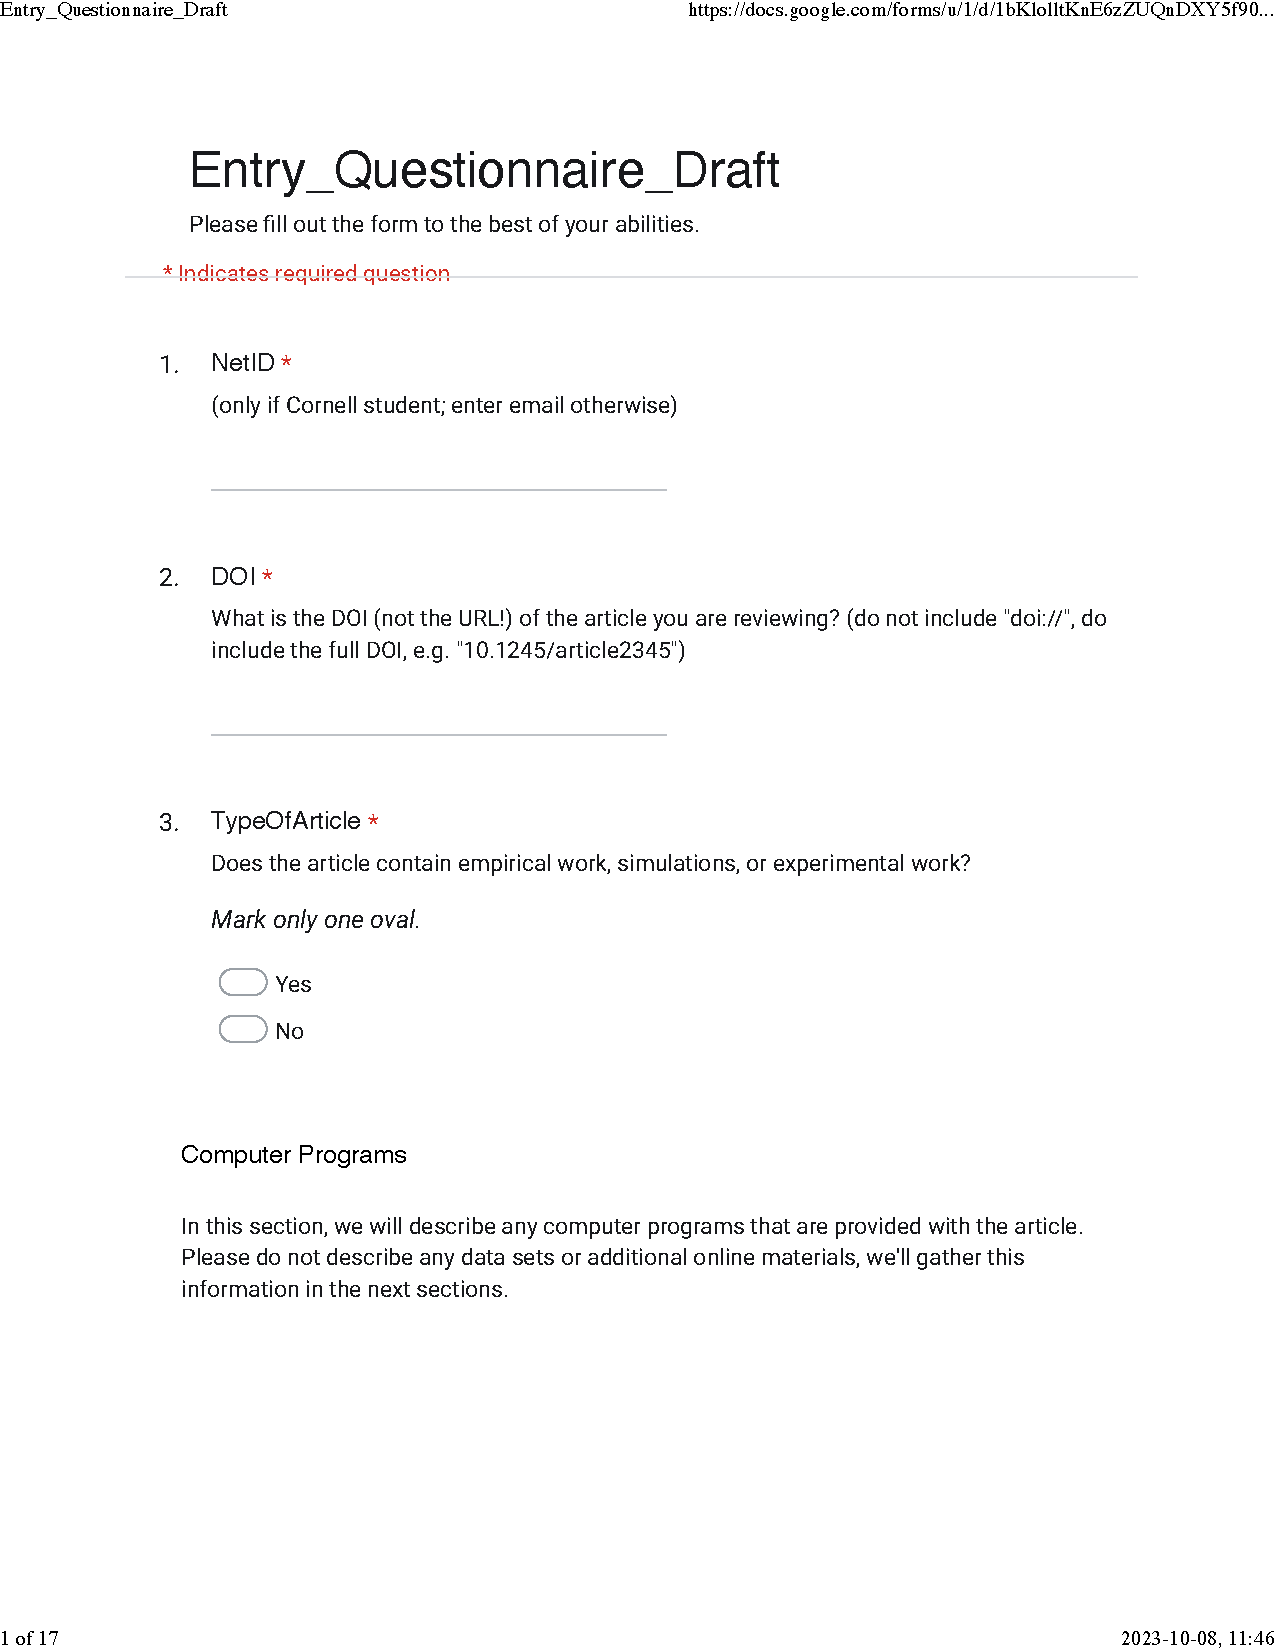
\includepdf[pages=1,scale=.8,pagecommand=\section{Assessment Questionnaire}\label{app:assessment_form}]{./includes/Entry_Questionnaire.pdf}
\includepdf[pages=2-,scale=.8,pagecommand={}]{./includes/Entry_Questionnaire.pdf}

% Exit Q
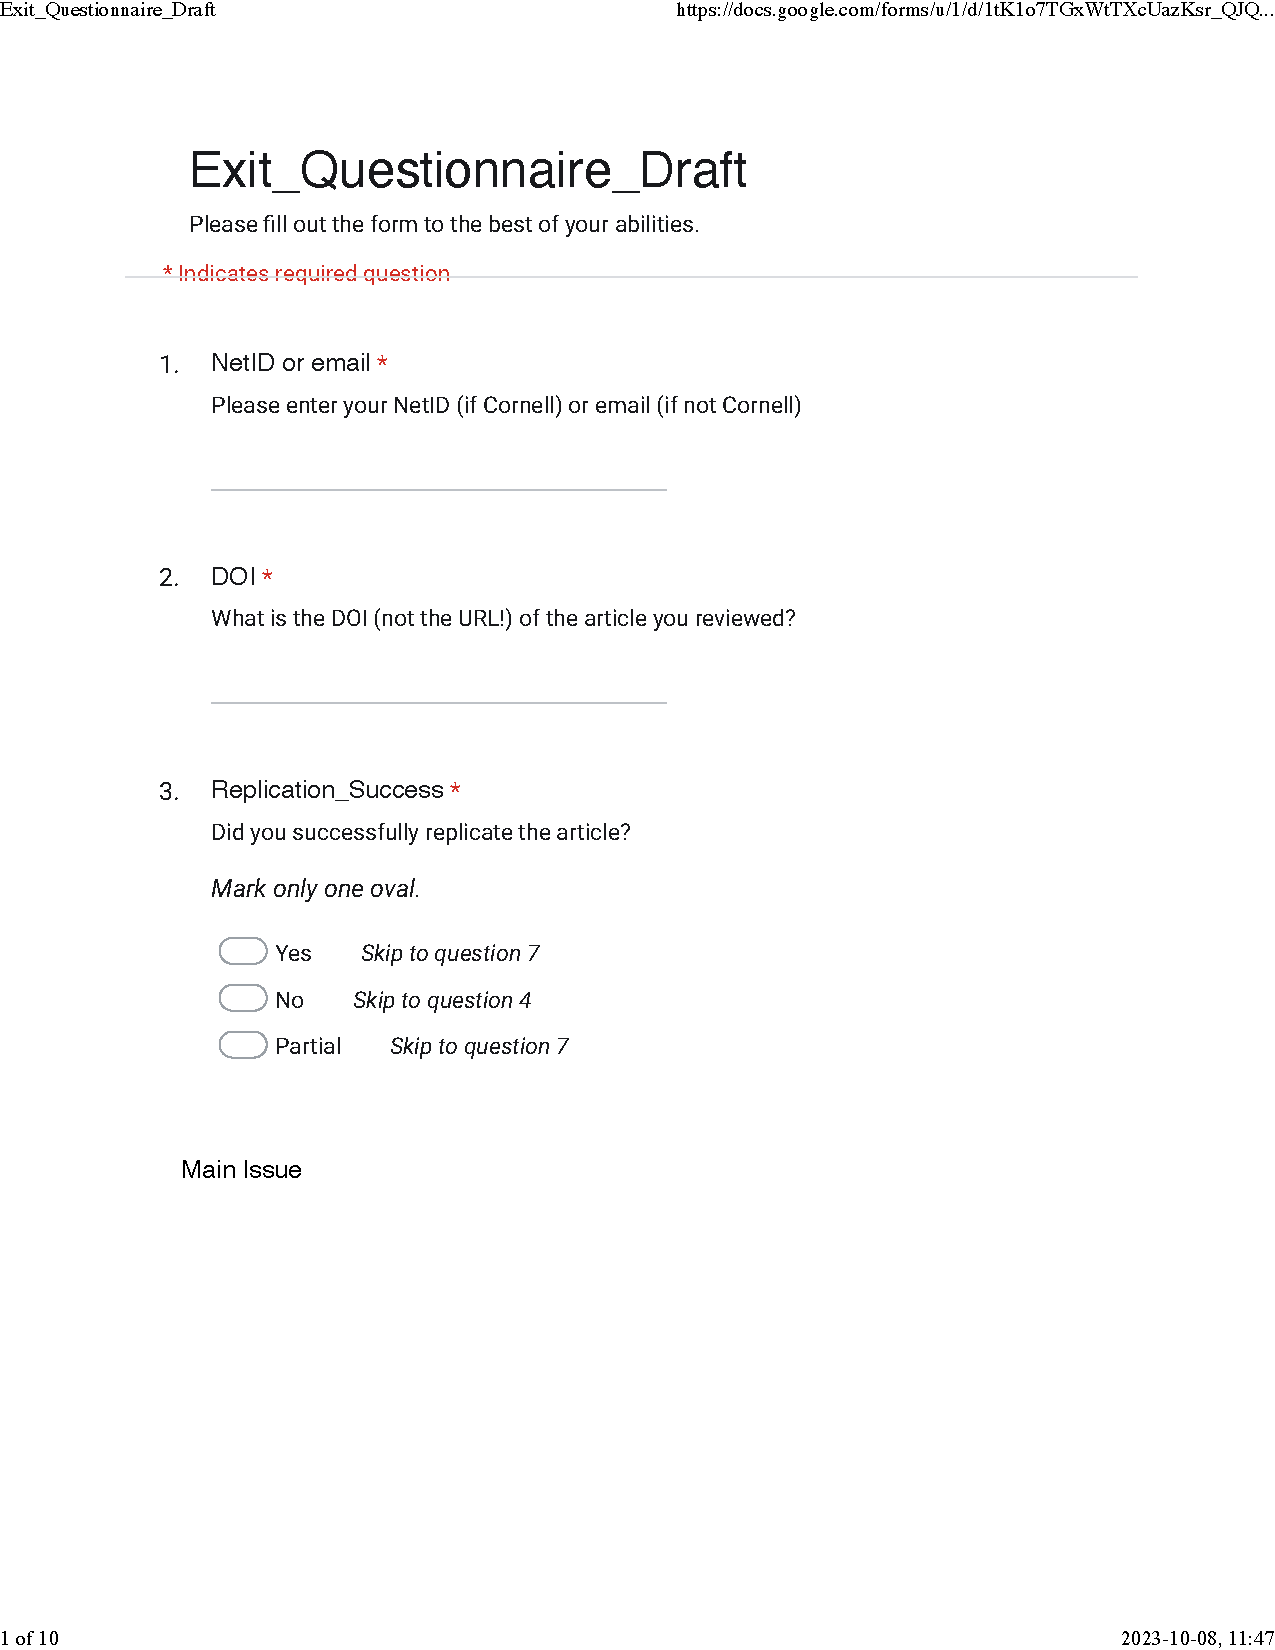
\includepdf[pages=1,scale=.8,pagecommand=\section{Exit Questionnaire}\label{app:exit_form}]{./includes/Exit_Questionnaire.pdf}
\includepdf[pages=2-,scale=.8,pagecommand={}]{./includes/Exit_Questionnaire.pdf}

\section{Replication Team}
The following members of the Replication Lab provided valuable assistance:

% first,initial,last,year
\csvreader[/csv/head=true,%
/csv/head to column names=true,%
/csv/late after line={,},%
/csv/late after last line=.,%
]%
{includes/Replication_Students_Historically.csv}{}{ \first \xspace \initial \xspace \last }

\newpage
\section{Acronyms Used}
% Define acronyms to be used in the text here. See
% http://www.mackichan.com/index.html?techtalk/456.htm~mainFrame for usage in
% Scientific workplace context

\begin{acronym}
\acro{ACS}{American Community Survey}
\acro{AEA}{American Economic Association}
\acro{AEJ:AE}{American Economic Journal: Applied Economics}
\acro{AEJ:Mac}{American Economic Journal: Macroeconomics}
\acro{AEJ:Mic}{American Economic Journal: Microeconomics}
\acro{AEJ:EP}{American Economic Journal: Economic Policy}
\acro{AER}{American Economic Review}
\acro{AJPS}{American Journal of Politial Science}
\acro{AHEAD}{Study of Assets and Health Dynamics Amongst the Oldest Old}
\acro{API}{application programming interface}
\acro{ASCII}{American Standard Code for Information  Interchange} %, typically used to denote raw text files in PC or Unix environments
\acro{ASM}{Annual Survey of Manufacturers}
\acro{BDS}{Business Dynamics Statistics}
\acro{BED}{Business Employment Dynamics}
\acro{BES}{Business Expenditure Survey}
\acro{BLS}{Bureau of Labor Statistics}
\acro{BRB}{Business Register Bridge}
\acro{BR}{Business Register}
\acro{CAC}{Cornell Center for Advanced Computing}
\acro{CBP}{County Business Patterns}
\acro{CBSA}{Core-Based Statistical Area}
\acro{CER}{Covered Earnings Records}
\acro{CES}{Center for Economic Studies}
\acro{CEW}{Covered Employment and Wages}%. Employment statistics program run by BLS in  conjunction with all states, also known as ES-202. Generally, when used  in this document, refers to public-use tabulations from the CEW, as  opposed to the confidential microdata received directly from the states.
\acro{CISER}{Cornell Institute for Social and Economic Research}
\acro{CIT}{Cornell Information Technologies}
\acro{CODA}{Children of Depression}
\acro{CPI}{Consumer Price Index}
\acro{CPI-U}{Consumer Price Index (All Urban Consumers)}
\acro{CPR}{Composite Person Record}
\acro{CPS}{Current Population Survey}
\acro{CRADC}{Cornell Restricted Access Data Center}
\acro{CTC}{Cornell Theory Center}
\acro{DCC}{Data Confidentiality Committee}
\acro{DOI}{Digital Object Identifier}
\acro{DER}{Detailed Earnings Record}
\acro{DRB}{Disclosure Review Board}
\acro{DWS}{Displaced Worker Supplement}
\acro{EJ}{Economic Journal}
\acro{ECF}{Employer Characteristics  File}
\acro{EHF}{Employment History Files}
%\acro{EIN}{\acroextra{(federal) }Employer Identification Number}
\acro{ERR}{Excess Reallocation Rate}
%\acro{ES-202}{ES-202\acroextra{. An older name for the \ac{QCEW} program}}
\acro{FHFA}{Federal Housing Finance Agency}
%\acro{FIPS}{Federal information processing standards codes\acroextra{\ issued     by \ac{NIST}}}
\acro{FSRDC}{Federal Statistical Research Data Center}
%\acro{FTI}{Federal Tax Information\acroextra{, typically covered under     Title 26, U.S.C.}}
\acro{GAL}{Geocoded Address List}
\acro{GIS}{Geographic Information System}
\acro{HPI}{House Price Index}
\acro{HRS}{Health and Retirement Study}
\acro{IAB}{Institute for Employment Research}
\acro{ICF}{Individual Characteristics File}
\acro{IRB}{Institutional Review Board}
\acro{IRS}{Internal Revenue Service}
\acro{ISR}{Institute for Social Research}
\acro{JCR}{Job Creation Rate}
\acro{JDR}{Job Destruction Rate}
\acro{JOLTS}{Job Openings and Labor Turnover Survey}
\acro{JASA}{Journal of the American Statistical Association}
\acro{JMCB}{Journal of Money, Credit and Banking}
\acro{JPE}{Journal of Political Economy}
\acro{JEEA}{Journal of the European Economic Association}
\acro{JRR}{Job Reallocation Rate}
\acro{LAUS}{Local Area Unemployment Statistics}
\acro{LBD}{Longitudinal Business Database}
%\acro{LDB}{\ac{BLS}'s Longitudinal Business Database}
\acro{LED}{Local Employment Dynamics}
\acro{LEHD}{Longitudinal Employer-Household Dynamics}
\acro{LMI}{Labor Market Information}
\acro{MBR}{Master Beneficiary Record}
\acro{MEF}{Master Earnings File}
\acro{MER}{Master Earnings Record}
\acro{MLS}{Mass Layoff Statistics}
\acro{MMS}{Methodology, Measurement, and Statistics}
\acro{MN}{Minnesota}
\acro{MSA}{Metropolitan Statistical Area}
\acro{MSD}{Metropolitan Statistical Division}
\acro{MWR}{Multiple Worksite Report}
\acro{NAICS}{North American Industry Coding System}
\acro{NECTA}{New England  City and Town Area}
\acro{NIA}{National Institute on Aging}
\acro{NIST}{National Institute of Standards and Technology}
\acro{NLSY}{National Longitudinal Study of Youth}
\acro{NSF}{National Science Foundation}
\acro{NSTA}{NAICS SIC Treatment of Auxiliaries}
\acro{OS}{operating system}
\acro{OTM}{OnTheMap}
\acro{PCF}{Person Characteristics File}
\acro{PHF}{Person History File}
\acro{PIK}{Protected Identity Key}
\acro{PSID}{Panel Study of Income Dynamics}
%\acro{QCEW}{Quarterly Census of Employment and Wages\acroextra{, managed by   the \acf{BLS}}}
\acro{QJE}{Quarterly Journal of Economics}
\acro{QWI}{Quarterly Workforce Indicators}
\acro{RDA}{Restricted Data Application}
\acro{RDC}{Research Data Center}
\acro{ReStat}{Review of Economics and Statistics}
\acro{RUN}{Reporting unit number}
%\acro{SEIN}{State employer identification number\acroextra{. It is     constructed from the state \ac{FIPS} code and the UI account     number. The BLS refers to the UI account number in combination with the     reporting unit number as SESA-ID}}
\acro{SEINUNIT}{SEIN reporting unit}
\acro{SEPB}{Summary of Earnings and Projected Benefits} % confidential SSA                                % file
%\acro{SESA-ID}{State Employment Security Agency ID\acroextra{. The UI     account number in combination with the Reporting Unit Number is treated   as a unique establishment identifier.}}
\acro{SESA}{State Employment Security Agency}
\acro{SIC}{Standard Industry Classification}
\acro{SIPP}{Survey of Income and Program Participation}
\acro{SLID}{Survey of Labour and Income Dynamics}
\acro{SPF}{Successor-Predecessor File}
\acro{SRMI}{Sequential Regression Multiple Imputation}
\acro{SSA}{Social Security Administration}
\acro{SSI}{Supplemental Security Income}
\acro{SSN}{Social Security Number}
\acro{SSR}{Supplemental Security Record}
%\acro{SynLBD}{Synthetic \ac{LBD}\acroextra{, a synthetic microdata file at the establishment level}}
\acro{U2W}{Unit-to-Worker Impute}
\acro{UI}{Unemployment Insurance}
\acro{URL}{Uniform Record Locator}
\acro{WB}{War Babies}
\acro{WIA}{Workforce Investment Act}
\acro{WIB}{Workforce Investment Board}
\acro{WRR}{Worker Reallocation Rate}
\acro{WTS}{Windows Terminal Services}
\acro{VCS}{version control system}
% Usage in the later text:
%  \ac{acronym}         Expand and identify the acronym the first time; use
%                       only the acronym thereafter
%  \acf{acronym}        Use the full name of the acronym.
%  \acs{acronym}        Use the acronym, even before the first corresponding
%                       \ac command
%  \acl{acronym}        Expand the acronym without using the acronym itself.
\end{acronym}

\clearpage
%Creation of reference list using .bib file
\bibliography{./includes/paper.bib}
\bibliographystyle{cjebibstyle} % to impose CJE bibliography style on output




\end{document}